% Préambule commun des schémas TikZ (compilés séparément par construire_figures.py)
\documentclass[tikz,border=3pt]{standalone}
\usepackage[T1]{fontenc}
\usepackage[utf8]{inputenc}
\usepackage{lmodern}
\usepackage{amsmath,amssymb}
\usepackage{bm}
\usepackage[american,siunitx,straightvoltages]{circuitikz}
\usetikzlibrary{arrows.meta,positioning,calc,decorations.pathmorphing,
  decorations.markings,decorations.pathreplacing,patterns,shapes.geometric,
  shapes.misc,shapes.multipart,fit,backgrounds,3d,intersections,matrix}

\ctikzset{bipoles/length=1.1cm, amplifiers/scale=0.85, tripoles/op amp/width=1.4}

\tikzset{
  >={Latex[length=2mm,width=1.4mm]},
  every picture/.style={line width=0.6pt, font=\small},
  % schémas-blocs
  bloc/.style={draw, minimum width=1.5cm, minimum height=0.9cm, align=center,
               inner sep=3pt, fill=white},
  somme/.style={draw, circle, minimum size=4.5mm, inner sep=0pt, fill=white,
                path picture={\draw (path picture bounding box.north west)
                  -- (path picture bounding box.south east)
                  (path picture bounding box.north east)
                  -- (path picture bounding box.south west);}},
  gain/.style={draw, isosceles triangle, isosceles triangle apex angle=60,
               minimum size=8mm, inner sep=1pt, fill=white},
  bruit/.style={draw, circle, minimum size=4.5mm, inner sep=0pt, fill=white,
                path picture={\node at (path picture bounding box.center)
                  {\scriptsize$\ast$};}},
  cadre/.style={draw, dashed, rounded corners=1pt},
  cadrept/.style={draw, dash dot, rounded corners=1pt},
  fleche/.style={->},
  % mécanique
  bati/.style={pattern=north east lines, draw=none},
  ressort/.style={decorate, decoration={coil, aspect=0.4, segment length=2.2mm,
                  amplitude=2mm, pre length=2mm, post length=2mm}},
  zigzag/.style={decorate, decoration={zigzag, segment length=2mm,
                  amplitude=1.6mm, pre length=2mm, post length=2mm}},
  pivot/.style={draw, circle, fill=white, minimum size=2.2mm, inner sep=0pt},
  masse/.style={draw, fill=gray!25, minimum width=1.4cm, minimum height=0.8cm},
  cote/.style={<->, line width=0.4pt},
  axe/.style={->, line width=0.6pt},
  trait mixte/.style={dash dot, line width=0.4pt},
}

% Encastrement / bâti hachuré : \bati{(x1,y1)}{(x2,y2)} trace une ligne et ses hachures dessous
\newcommand{\bati}[3][0.18]{%
  \fill[pattern=north east lines] #2 rectangle ($#3+(0,-#1)$);
  \draw[line width=0.8pt] #2 -- #3;}

% Transducteur (deux cercles entrelacés) : \pic (t) at (x,y) {transducteur};  -> (t-o) entrée, (t-e) sortie
\tikzset{
  transducteur/.pic={\draw (-0.13,0) circle (0.24); \draw (0.13,0) circle (0.24);
    \coordinate (-o) at (-0.37,0); \coordinate (-e) at (0.37,0);
    \coordinate (-n) at (0,0.24); \coordinate (-s) at (0,-0.24);},
  bobine/.style={decorate, decoration={coil, aspect=0.7, segment length=1.4mm,
                 amplitude=1.6mm, pre length=1mm, post length=1mm}},
  sourcebruit/.style={draw, circle, minimum size=5mm, inner sep=0pt, fill=white,
                 label={[inner sep=0pt]center:$\ast$}},
  sourcecourant/.style={draw, circle, minimum size=5mm, inner sep=0pt, fill=white,
                 label={[inner sep=0pt]center:$\circledast$}},
}

% Composants compacts (pour les petits boîtiers des schémas-blocs)
\newcommand{\resistance}[2]{% de #1 à #2 (quelconque)
  \draw #1 -- ($#1!0.22!#2$) ($#1!0.78!#2$) -- #2;
  \draw[decorate, decoration={zigzag, segment length=1.5mm, amplitude=1.1mm}]
    ($#1!0.22!#2$) -- ($#1!0.78!#2$);}
\newcommand{\condensateur}[2]{% horizontal de #1 à #2
  \draw #1 -- ($($#1!0.5!#2$)+(-0.05,0)$) ($($#1!0.5!#2$)+(0.05,0)$) -- #2;
  \draw[line width=1pt] ($($#1!0.5!#2$)+(-0.05,0.14)$) -- ($($#1!0.5!#2$)+(-0.05,-0.14)$)
                        ($($#1!0.5!#2$)+(0.05,0.14)$) -- ($($#1!0.5!#2$)+(0.05,-0.14)$);}
% R // C horizontal : \RparC{(x,y)}{longueur}{écart}  (centre, longueur totale, écart vertical)
\newcommand{\RparC}[3]{%
  \coordinate (rcA) at ($#1+(-#2/2,0)$); \coordinate (rcB) at ($#1+(#2/2,0)$);
  \draw (rcA) -- ++(0.15,0) coordinate (rcA1) (rcB) -- ++(-0.15,0) coordinate (rcB1);
  \draw (rcA1) -- ++(0,#3/2) (rcA1) -- ++(0,-#3/2) (rcB1) -- ++(0,#3/2) (rcB1) -- ++(0,-#3/2);
  \resistance{($(rcA1)+(0,#3/2)$)}{($(rcB1)+(0,#3/2)$)}
  \condensateur{($(rcA1)+(0,-#3/2)$)}{($(rcB1)+(0,-#3/2)$)}}

\begin{document}
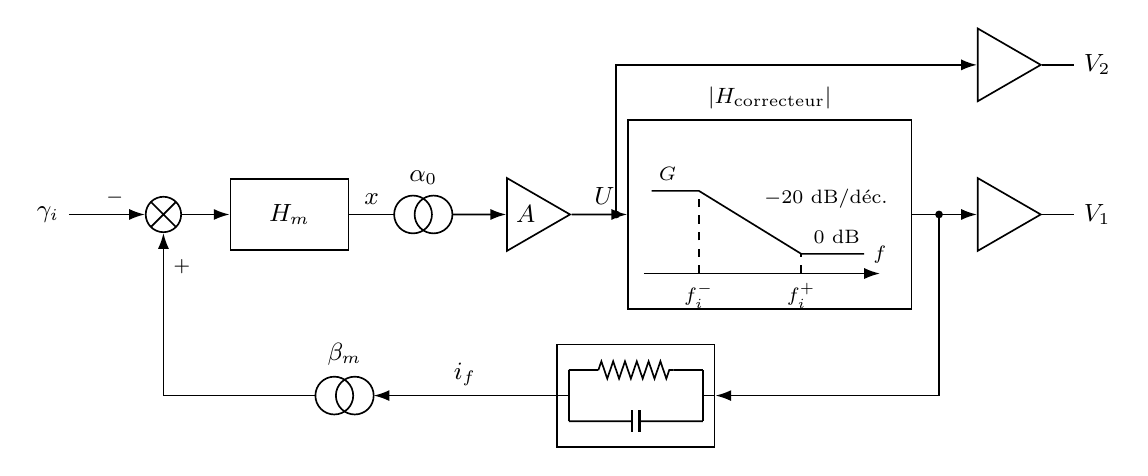
\begin{tikzpicture}[font=\small]
  \node[somme] (s) at (0,0) {};
  \node[bloc] (h) at (1.6,0) {$H_m$};
  \pic (t) at (3.3,0) {transducteur}; \node[above=2.5mm] at (3.3,0) {$\alpha_0$};
  \node[gain] (a) at (4.6,0) {$A$};
  \node[bloc, minimum width=3.6cm, minimum height=2.4cm] (cor) at (7.7,0) {};
  \begin{scope}[shift={(6.1,-0.75)}]
    \draw[->] (0,0) -- (3.0,0) node[above, font=\scriptsize] {$f$};
    \draw (0.1,1.05) -- (0.7,1.05) -- (2.0,0.25) -- (2.8,0.25);
    \draw[dashed] (0.7,0) -- (0.7,1.05) (2.0,0) -- (2.0,0.25);
    \node[above, font=\scriptsize] at (0.3,1.05) {$G$};
    \node[font=\scriptsize, anchor=west] at (1.4,0.95) {$-20$ dB/déc.};
    \node[above, font=\scriptsize] at (2.45,0.25) {0 dB};
    \node[below, font=\scriptsize] at (0.7,0) {$f_i^-$}; \node[below, font=\scriptsize] at (2.0,0) {$f_i^+$};
  \end{scope}
  \node[above, font=\footnotesize] at (cor.north) {$|H_{\text{correcteur}}|$};
  \node[gain] (v1) at (10.6,0) {};
  \node[gain] (v2) at (10.6,1.9) {};
  \draw[->] (-1.2,0) node[left] {$\gamma_i$} -- (s) node[above left, pos=0.85] {\scriptsize$-$};
  \draw[->] (s) -- (h); \draw (h) -- node[above] {$x$} (t-o); \draw[->] (t-e) -- (a);
  \draw[->] (a) -- (cor); \node[above] at (5.6,0) {$U$};
  \fill (5.75,0) circle (1.4pt);
  \draw[->] (5.75,0) |- (v2);
  \draw[->] (cor) -- (v1);
  \draw (v1.east) -- ++(0.4,0) node[right] {$V_1$};
  \draw (v2.east) -- ++(0.4,0) node[right] {$V_2$};
  % contre-réaction
  \coordinate (n) at (9.85,0); \fill (n) circle (1.4pt);
  \node[bloc, minimum width=2.0cm, minimum height=1.3cm] (rc) at (6.0,-2.3) {};
  \RparC{(6.0,-2.3)}{2.0}{0.65}
  \pic (b) at (2.3,-2.3) {transducteur}; \node[above=2.5mm] at (2.3,-2.3) {$\beta_m$};
  \draw[->] (n) |- (rc.east);
  \draw[->] (rc.west) -- node[above] {$i_f$} (b-e);
  \draw[->] (b-o) -| (s.south) node[below right, pos=0.95] {\scriptsize$+$};
\end{tikzpicture}
\end{document}
